\documentclass[tikz, border=10pt]{standalone}
\usetikzlibrary{automata, positioning, arrows}

\begin{document}

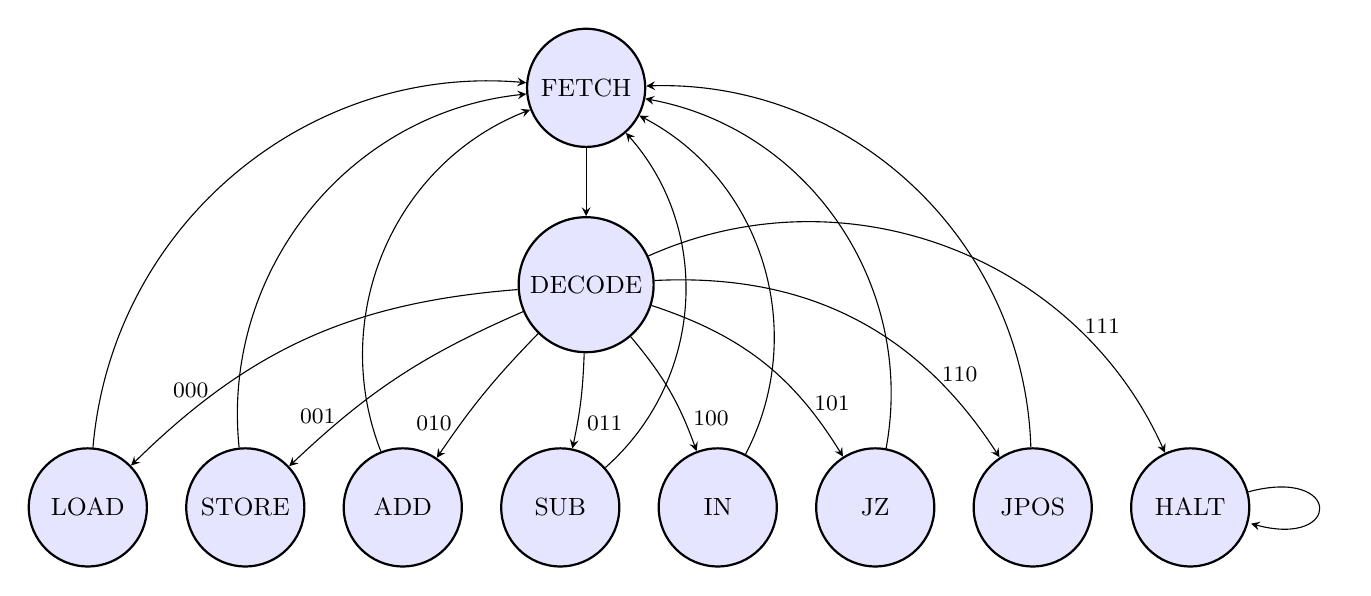
\begin{tikzpicture}[
    ->, >=stealth, auto, node distance=2.5cm,
    every state/.style={thick, fill=blue!10, minimum size=1.5cm, font=\small},
    initial text=$ $
]

    % Top Level
    \node[state] (FETCH) {FETCH};
    
    % Second Level
    \node[state, below of=FETCH, node distance=2.5cm] (DECODE) {DECODE};
    
    % Execution States
    % Group 1: Memory Operations (000-011)
    \node[state, below left of=DECODE, node distance=4cm, xshift=-3.5cm] (LOAD) {LOAD};
    \node[state, right of=LOAD, node distance=2cm] (STORE) {STORE};
    \node[state, right of=STORE, node distance=2cm] (ADD) {ADD};
    \node[state, right of=ADD, node distance=2cm] (SUB) {SUB};
    
    % Group 2: IO & Flow Control (100-111)
    \node[state, right of=SUB, node distance=2cm] (IN) {IN};
    \node[state, right of=IN, node distance=2cm] (JZ) {JZ};
    \node[state, right of=JZ, node distance=2cm] (JPOS) {JPOS};
    \node[state, right of=JPOS, node distance=2cm] (HALT) {HALT};


    % Edges
    % Fetch -> Decode
    \path (FETCH) edge node {} (DECODE);
    
    % Decode -> Operations
    \path (DECODE) edge [bend right=20] node [left, near end, font=\footnotesize] {000} (LOAD)
          (DECODE) edge [bend right=10] node [left, near end, font=\footnotesize] {001} (STORE)
          (DECODE) edge [bend right=5] node [left, near end, font=\footnotesize] {010} (ADD)
          (DECODE) edge [bend left=5] node [right, near end, font=\footnotesize] {011} (SUB)
          (DECODE) edge [bend left=10] node [right, near end, font=\footnotesize] {100} (IN)
          (DECODE) edge [bend left=20] node [right, near end, font=\footnotesize] {101} (JZ)
          (DECODE) edge [bend left=30] node [right, near end, font=\footnotesize] {110} (JPOS)
          (DECODE) edge [bend left=45] node [right, near end, font=\footnotesize] {111} (HALT);

    % Operations -> Fetch (Return)
    \path (LOAD)   edge [bend left=45] node {} (FETCH)
          (STORE)  edge [bend left=45] node {} (FETCH)
          (ADD)    edge [bend left=45] node {} (FETCH)
          (SUB)    edge [bend right=45] node {} (FETCH)
          (IN)     edge [bend right=45] node {} (FETCH)
          (JZ)     edge [bend right=45] node {} (FETCH)
          (JPOS)   edge [bend right=45] node {} (FETCH);
          
    % Halt Loop
    \path (HALT)   edge [loop right] node {} (HALT);

\end{tikzpicture}

\end{document}
